% !TEX program = pdflatex
% =====================================================================
%  ViT-JAX Distributed Scaling  —  5-minute in-class presentation
%  Michael Wang  ·  Team Tensor  ·  CS 390: Distributed Systems  ·  Duke, Spring 2026
%
%  Compile:  pdflatex 5min_presentation.tex   (run twice)
%  Theme:    metropolis (modern, minimal; ships with TeX Live 2019+)
%
%  Structure: 6 frames, ~4 min of talking + ~1 min buffer for transitions/Q&A.
%  Every bullet reveals on a click — see \item<+-> and \onslide<+-> markers.
%  Speaker-facing timing comments precede each frame (not rendered on slides).
% =====================================================================
\documentclass[aspectratio=169,10pt]{beamer}

\usetheme{metropolis}
\usepackage{appendixnumberbeamer}
\usepackage{booktabs}
\usepackage{graphicx}
\usepackage{amsmath,amssymb}
\usepackage{xcolor}
\usepackage{tikz}
\usetikzlibrary{arrows.meta, positioning, shapes.geometric, fit, backgrounds}

\graphicspath{{../outputs/}{../outputs/scaling/}{../outputs/straggler/}%
              {../outputs/training/100_epoch/}}

\definecolor{accent}{HTML}{2563EB}
\definecolor{warn}{HTML}{D97706}
\definecolor{muted}{HTML}{6B7280}
\setbeamercolor{alerted text}{fg=accent}

\title{ViT-JAX Distributed Scaling}
\subtitle{Data-parallel Vision Transformer training on TPU v6e-8\\\textit{Scaling behaviour \& straggler tax}}
\author{Michael Wang \\ \textit{\small Team Tensor}}
\institute{CS 390 — Distributed Systems · Duke University}
\date{Spring 2026}

\begin{document}

% ---------------------------------------------------------------------
% Timing: 0:00–0:05  (5 s)
% Speaker cue: name + team + title + one-breath intro. Do NOT linger here.
%   "Hi — I'm Michael from Team Tensor. This is ViT-JAX Distributed
%    Scaling: a systems study of data-parallel training on TPU v6e-8."
% ---------------------------------------------------------------------
\begin{frame}[plain]
  \titlepage
\end{frame}

% ---------------------------------------------------------------------
% Timing: 0:05–0:45  (40 s)  |  Clicks: 5  |  Trimmed 5 s from
%         headline click to buy time for the model bullets.
% Speaker cues:
%   (0, ~11 s) Scene: systems study, not accuracy study.
%   (1, ~6 s)  "Experiment 1: throughput vs device count."
%   (2, ~6 s)  "Experiment 2: what one slow chip costs the cluster."
%   (3, ~9 s)  "Headline: 100 epochs, 421 s, 55% top-1, ~15k img/s."
%   (4, ~4 s)  "Not SOTA — goal is distributed behaviour."
% ---------------------------------------------------------------------
\begin{frame}{What I built and why}
  \begin{columns}[T,onlytextwidth]
    \begin{column}{0.56\textwidth}
      \textbf{A systems study of synchronous data parallelism}, using
      ViT-Small (9.55\,M params) on CIFAR-100 in JAX/Flax, running on
      TPU v6e-8 (8 chips, bf16).

      \vspace{0.6em}
      Two experiments on the same testbed:
      \begin{enumerate}[<+->]\small
        \item \textbf{Scaling} — how throughput grows with device count.
        \item \textbf{Stragglers} — what one slow chip costs the cluster.
      \end{enumerate}

      \vspace{0.6em}
      \onslide<+->{\textbf{Headline training run:}
      \begin{itemize}\small
        \item 100 epochs in \alert{421\,s}
        \item \alert{55.04\,\%} top-1, \alert{80.18\,\%} top-5
        \item $\approx$\,15\,000 images/sec sustained
      \end{itemize}}

      \vspace{0.4em}
      \onslide<+->{\textcolor{muted}{\footnotesize Not a SOTA attempt — the goal is to
      \emph{measure} distributed behaviour.}}
    \end{column}
    \begin{column}{0.42\textwidth}
      \begin{center}
        \includegraphics[width=\linewidth,height=0.72\textheight,keepaspectratio]%
          {training/100_epoch/training_curves.png}
        \\[-0.2em]
        {\scriptsize\textcolor{muted}{Train/test loss \& accuracy, 100 epochs.}}
      \end{center}
    \end{column}
  \end{columns}
\end{frame}

% ---------------------------------------------------------------------
% Timing: 0:50–1:35  (45 s)  |  Clicks: 3  |  Trimmed from 50 s to
%                              buy back time for the model bullets.
% Speaker cues:
%   (diagram visible at start — 6 s: describe the flow left-to-right,
%    batch → shard → 8 devices → pmean barrier → update.)
%   (1, ~10 s) "Replicate, shard, compute, all-reduce, update — one step."
%   (2, ~8 s)  "Mathematically identical to 1-chip training, full batch.
%               pmean averages the gradients."
%   (3, ~10 s) "The key: every device must reach pmean before any can
%               proceed. That barrier is what both experiments probe."
% ---------------------------------------------------------------------
\begin{frame}{How one training step becomes distributed}
  \vspace{-0.4em}
  \begin{center}
  \resizebox{\linewidth}{!}{%
  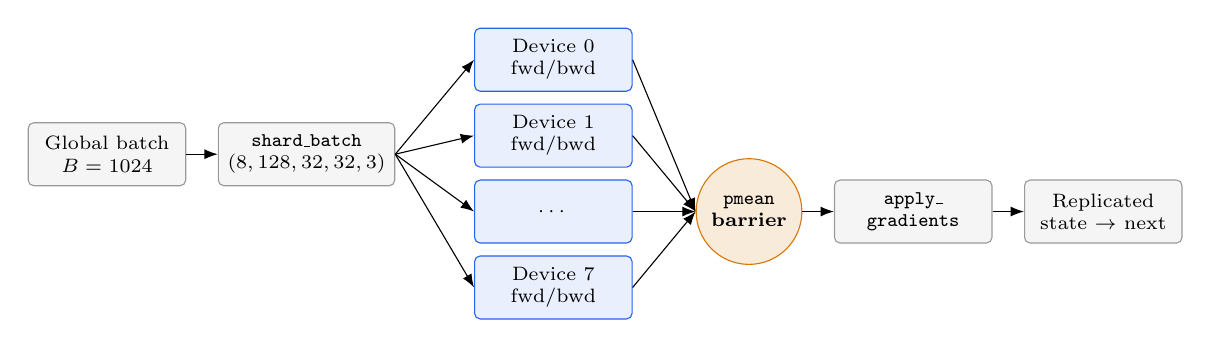
\begin{tikzpicture}[
      >=Latex, node distance=4mm,
      box/.style={rounded corners=2pt, draw=black!40, fill=gray!8,
                  minimum width=20mm, minimum height=8mm, font=\scriptsize,
                  align=center},
      dev/.style={rounded corners=2pt, draw=accent, fill=accent!10,
                  minimum width=20mm, minimum height=8mm, font=\scriptsize,
                  align=center},
      barrier/.style={circle, draw=warn, fill=warn!15, minimum size=11mm,
                      font=\scriptsize\bfseries, align=center},
    ]
    \node[box]  (batch) {Global batch\\$B=1024$};
    \node[box, right=of batch] (shard) {\texttt{shard\_batch}\\$(8,128,32,32,3)$};

    \node[dev, right=10mm of shard, yshift=12mm]  (d0) {Device 0\\fwd/bwd};
    \node[dev, below=1.5mm of d0]                 (d1) {Device 1\\fwd/bwd};
    \node[dev, below=1.5mm of d1]                 (dd) {$\cdots$};
    \node[dev, below=1.5mm of dd]                 (d7) {Device 7\\fwd/bwd};

    \node[barrier, right=8mm of dd] (pm) {\texttt{pmean}\\barrier};

    \node[box, right=of pm] (upd) {\texttt{apply\_}\\\texttt{gradients}};
    \node[box, right=of upd] (next) {Replicated\\state $\to$ next};

    \draw[->] (batch) -- (shard);
    \draw[->] (shard.east) -- (d0.west);
    \draw[->] (shard.east) -- (d1.west);
    \draw[->] (shard.east) -- (dd.west);
    \draw[->] (shard.east) -- (d7.west);
    \draw[->] (d0.east) -- (pm.west);
    \draw[->] (d1.east) -- (pm.west);
    \draw[->] (dd.east) -- (pm.west);
    \draw[->] (d7.east) -- (pm.west);
    \draw[->] (pm) -- (upd);
    \draw[->] (upd) -- (next);
  \end{tikzpicture}}%
  \end{center}

  \vspace{-0.4em}
  {\raggedright\begin{itemize}[<+->]\small
    \item \textbf{Replicate} params, \textbf{shard} batch, \textbf{compute} local grads,
          \textbf{all-reduce} via \texttt{pmean}, \textbf{update} identically.
    \item Mathematically equivalent to single-device training with the full global batch.
    \item \alert{Every device must reach \texttt{pmean} before any can proceed.}
          That barrier is what both experiments probe.
  \end{itemize}\par}
\end{frame}

% ---------------------------------------------------------------------
% Timing: 1:45–2:50  (65 s)  |  Clicks: 5  |  Plot + setup visible at start.
% Speaker cues (see 5min_script.md for full prose):
%   (entry, ~10 s): describe plot — y = fraction of perfect scaling.
%   (1, ~9 s):  "k=2 → 0.87, near-perfect."
%   (2, ~11 s): "k=8 → 0.36; 8× hardware but only 2.9× speedup."
%   (3, ~12 s): "Cause: 1024 split 8 ways = 128/chip, MXU starves."
%   (4, ~8 s):  MODEL reveal — T_k = T_1/k + R log_2 k,
%               R=11.5 ms fits η at all three k within 2 pp. ✓
%   (5, ~5 s):  Punchline — "batch-size trap."
% ---------------------------------------------------------------------
\begin{frame}{Does 8$\times$ chips really mean 8$\times$ faster training?}
  \begin{columns}[T,onlytextwidth]
    \begin{column}{0.55\textwidth}
      \includegraphics[width=\linewidth,height=0.78\textheight,keepaspectratio]%
        {scaling/scaling_efficiency_vs_devices.png}
    \end{column}
    \begin{column}{0.45\textwidth}
      \small
      \textbf{Setup.} Fixed global batch (1024). Sweep $k = 1, 2, 4, 8$ chips.
      Plot the fraction of \emph{perfect} scaling achieved ($\eta = 1.0$ = ideal).

      \vspace{0.5em}
      \begin{itemize}[<+->]\footnotesize
        \item \textbf{k=2:} $\eta = 0.87$ — near-linear.
        \item \textbf{k=8:} $\eta$ crashes to \alert{0.36}. 8$\times$ hardware, only \alert{2.9$\times$} speedup.
        \item \textbf{Cause:} per-chip batch shrinks $1024 \to 128$ — MXU starves.
        \item \textbf{Model:}\; $T_k = \dfrac{T_1}{k} + R\log_2 k$,\; $R = 11.5$ ms/doubling\\[2pt]
              Predicted $\eta_{2/4/8} = 0.87 / 0.63 / 0.36$;
              measured $0.87 / 0.65 / 0.36$ \checkmark
      \end{itemize}

      \vspace{0.4em}
      \onslide<+->{\textcolor{accent}{\small \textbf{Takeaway:} strong scaling
      (fixed global batch) is a batch-size trap.}}
    \end{column}
  \end{columns}
\end{frame}

% ---------------------------------------------------------------------
% Timing: 2:50–3:55  (65 s)  |  Clicks: 5  |  Plot + setup visible at start.
% Speaker cues (see 5min_script.md for full prose):
%   (entry, ~10 s): describe plot — slowdown as extra work on chip 0.
%   (1, ~9 s):  "5k iters on chip 0 → whole cluster 1.1× slower."
%   (2, ~12 s): "200k iters → 3.33× cluster slowdown; 19.8k → 5.9k img/s."
%   (3, ~12 s): "Why: pmean barrier; 7 chips idle waiting for chip 0."
%   (4, ~8 s):  MODEL reveal — barrier = max-over-devices;
%               σ(δ) = 1 + τδ/T_base. σ(100k)=2.17 vs 2.14 ✓
%   (5, ~5 s):  Punchline — "only as fast as slowest chip."
% ---------------------------------------------------------------------
\begin{frame}{What does \emph{one} slow chip cost the whole cluster?}
  \begin{columns}[T,onlytextwidth]
    \begin{column}{0.55\textwidth}
      \includegraphics[width=\linewidth,height=0.78\textheight,keepaspectratio]%
        {straggler/slowdown_vs_delay.png}
    \end{column}
    \begin{column}{0.45\textwidth}
      \small
      \textbf{Setup.} Inject extra matmul work on \emph{device 0 only}.
      Measure step time of the whole 8-chip cluster. Baseline step = 52\,ms.

      \vspace{0.5em}
      \begin{itemize}[<+->]\footnotesize
        \item Small injection (5k iters): cluster \alert{$1.1\times$} slower.
        \item Big injection (200k iters): cluster \alert{$3.33\times$} slower.
              Throughput $19.8\text{k} \to 5.9\text{k}$ img/s.
        \item \textbf{Cause:} \texttt{pmean} is a sync barrier — 7 chips sit \emph{idle}
              waiting for chip 0.
        \item \textbf{Model:}\;
              $\sigma(\delta) = 1 + \dfrac{\tau \delta}{T_{\text{base}}}$,\;
              $\tau \approx 0.6\,\mu$s/iter\\[2pt]
              Predicted $\sigma(100\text{k}) = 2.17$; measured $2.14$ \checkmark
      \end{itemize}

      \vspace{0.4em}
      \onslide<+->{\textcolor{accent}{\small \textbf{Takeaway:} a cluster is only
      as fast as its slowest chip.}}
    \end{column}
  \end{columns}
\end{frame}

% ---------------------------------------------------------------------
% Timing: 3:30–4:00  (30 s)  |  Clicks: 3  |  Then ~60 s Q&A buffer
% Speaker cues:
%   (1) "Takeaway one: strong scaling is a small-batch trap — we lose
%        2.78× of the ideal speedup going 1 to 8 chips, purely from
%        compute starvation."
%   (2) "Takeaway two: the barrier really is the barrier — one slow
%        device, three orders of magnitude below a real fault,
%        slows everything 3.33×."
%   (3) "Thanks — happy to take questions."  [open Q&A]
% ---------------------------------------------------------------------
\begin{frame}{Takeaways}
  \begin{enumerate}[<+->]\small
    \item \textbf{Strong scaling is a small-batch trap.} Going $1\to8$ chips loses
          \alert{$2.78\times$ of the ideal speedup} as per-device batch collapses and
          the MXU starves.
    \item \textbf{The barrier really is the barrier.} One slow chip
          \alert{slows the cluster $3.33\times$} — seven of eight devices sit idle at
          \texttt{pmean}. The argument for async-SGD, backup workers, elastic training.
  \end{enumerate}

  \vspace{0.4em}
  \onslide<+->{%
    \begin{center}
      \textbf{Thank you — questions?}\\[0.2em]
      \textcolor{muted}{\small
      Repo: \texttt{github.com/Michael-OvO/vit-jax-distributed-scaling}}
    \end{center}%
  }
\end{frame}

\end{document}
